\icode{N24E-MCH-SI-L2-261026-001}
\nceeID[4]{2024湖北}{3}
如图所示，有五片荷叶伸出荷塘水面，一只青蛙要从高处荷叶跳到低处荷叶上，设低处荷叶 \(a\)、\(b\)、\(c\)、\(d\) 和青蛙在同一竖直平面内，\(a\)、\(b\) 高度相同，\(c\)、\(d\) 高度相同，\(a\)、\(b\) 分别在 \(c\)、\(d\) 正上方。将青蛙的跳跃视为平抛运动，若以最小的初速度完成跳跃，则它应跳到\paren[]

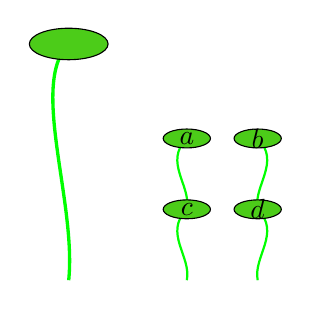
\begin{tikzpicture}
	\begin{scope}
		\draw[very thick,green] (0,0)..controls(-.5,-.5)and(.1,-2)..(0,-3);
		\draw[fill=green!60!brown] (0,0) ellipse(.5 and .2);
	\end{scope}
	\begin{scope}[scale=.6,xshift=2.5cm,yshift=-2cm]
		\draw[thick,green] (0,0)..controls(-.5,-.5)and(.1,-1)..(0,-1.5);
		\draw[fill=green!60!brown] (0,0) ellipse(.5 and .2);
		\node at(0,0){ \(a\)};
	\end{scope}
	\begin{scope}[scale=.6,xshift=2.5cm,yshift=-3.5cm]
		\draw[thick,green] (0,0)..controls(-.5,-.5)and(.1,-1)..(0,-1.5);
		\draw[fill=green!60!brown] (0,0) ellipse(.5 and .2);
		\node at(0,0){ \(c\)};
	\end{scope}
	\begin{scope}[scale=.6,xshift=4cm,yshift=-2cm]
		\draw[thick,green] (0,0)..controls(.5,-.5)and(-.1,-1)..(0,-1.5);
		\draw[fill=green!60!brown] (0,0) ellipse(.5 and .2);
		\node at(0,0){ \(b\)};
	\end{scope}
	\begin{scope}[scale=.6,xshift=4cm,yshift=-3.5cm]
		\draw[thick,green] (0,0)..controls(.5,-.5)and(-.1,-1)..(0,-1.5);
		\draw[fill=green!60!brown] (0,0) ellipse(.5 and .2);
		\node at(0,0){ \(d\)};
	\end{scope}
\end{tikzpicture}
\begin{choices}
	\item 荷叶\(a\)
	\item 荷叶\(b\)
	\item 荷叶\(c\)
	\item 荷叶\(d\)
\end{choices}
\begin{answer}
	C\qquad 提示：竖直高度最大，水平距离最小，速度最小
\end{answer}